\documentclass[tikz,border=3.14pt]{standalone}

%Stack overflow for cloud rect
\newcommand*{\StartSegmentLength}{8pt}
\usetikzlibrary{3d,decorations.text,shapes.arrows,positioning,fit,backgrounds,shapes.geometric,calc,decorations.markings,arrows,shapes.symbols,decorations.pathmorphing}

\tikzstyle{every pin edge}=[thick]
\tikzstyle{label distance}=[0.2cm]
\tikzset{
    aligned pin/.style args={[#1,#2,#3,#4]#5:#6}{
        pin={[inner sep=0pt,%
            pin distance=#2,% new option, default = 3ex
            very thick,
            label={[append after command={%
                    node[%
                        inner sep=0pt,%
                        xshift=#3,% modified, default = 0
                        yshift=#4,% modified, default = 0
                        at=(\tikzlastnode.#5),%
                        anchor=#1,%
                        draw opacity=0,
                        black,
                        font=\tiny,
                        align=center,
                    ]{#6}%
                }%
            ]center:{}}%
        ]#5:{}}%
    }
}

\definecolor{forestgreen}{rgb}{0,0.3,0.05}
\definecolor{alloyorange}{rgb}{0.77,0.38,0.06}
\definecolor{acidgreen}{rgb}{0.69,0.75,0.1}
\definecolor{pppizzaz}{rgb}{1,0.2,1}
\definecolor{fblue}{rgb}{0,0.47,0.7}
\definecolor{bred}{rgb}{0.3,0,0.05}
\definecolor{bpp}{rgb}{0.15,0,0.3}
\definecolor{gyellow}{rgb}{0.53,1,0.3}
\definecolor{salmon}{rgb}{1,0.58,0.5}
\definecolor{zbrown}{rgb}{0.2,0.2,0}
\definecolor{tblue}{rgb}{0.13,0.43,0.46}


\begin{document}

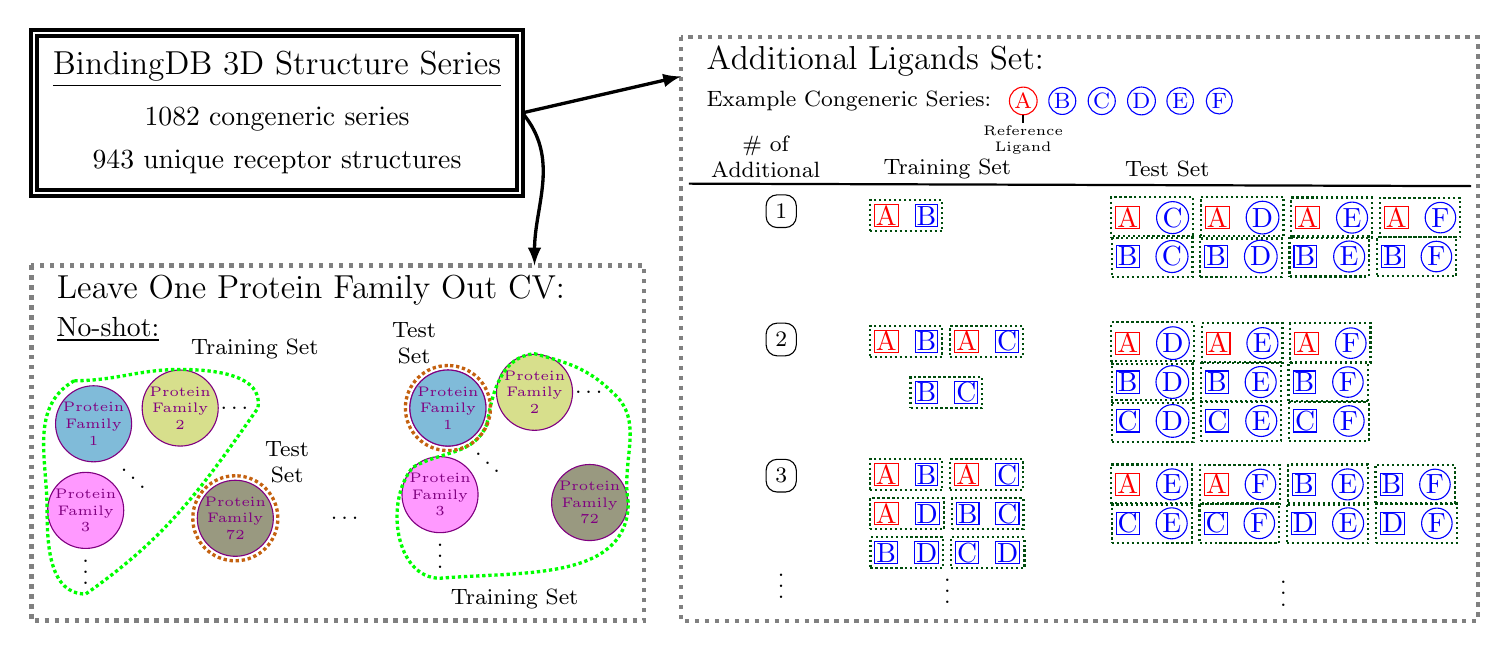
\begin{tikzpicture}        
        % \node[anchor=west,font=\huge] (datasets) at (0,1){Datasets};
        \begin{scope}[shift={(0,0.0)}]
                \node[anchor=west,text ragged,font=\large] (bdb) at ($(0,1)+(0.2,-0.5cm)$) {\underline{BindingDB 3D Structure Series}};
                \node[anchor=west,below=0cm of bdb] (bdb_cong) {1082 congeneric series};
                \node[anchor=west,below=0cm of bdb_cong] (bdb_rec) {943 unique receptor structures};
                \node[fit=(bdb) (bdb_rec),draw,rectangle,ultra thick,double] (bdb border) {};
        \end{scope}

        %Additional Ligands Evaluation
        \begin{scope}[every node/.style={node distance=0.5cm,font=\footnotesize},shift={(8.5,1.6)}]
                \node[anchor=west,font=\large] (addnleval) at (0,-1){Additional Ligands Set:};
                \node[anchor=west] (congser) at (0,-1.5){Example Congeneric Series:};  
                \node[circle,anchor=west,draw,red,inner sep=0.2mm,right=0.1cm of congser,aligned pin={[north,1mm,0,.14cm]270:Reference\\ Ligand}] (ref) {A};
                \foreach \letter/\place in {B/1,C/2,D/3,E/4,F/5}
                \node[circle,draw,blue,anchor=west,inner sep=0.2mm] (ref\place) at ($(ref.west) + (\place*0.5,0)$){\letter};

                \node[anchor=south west,text width=1.5cm,text centered,font=\footnotesize] (addnl) at (0,-2.6){\# of Additional};
                \begin{scope}[every node/.style={node distance=1.2cm,anchor=west},shift={(addnl.south)}]
                        \node[rectangle,draw,rounded corners,text centered,font=\footnotesize] (1addnl) at (0,-0.3){1};
                        \node[rectangle,draw,rounded corners,text centered,font=\footnotesize,below=of 1addnl] (2addnl) {2};
                        \node[rectangle,draw,rounded corners,text centered,font=\footnotesize,below=1.3cm of 2addnl] (3addnl) {3};
                        \node[text centered,font=\footnotesize,below=0.7cm of 3addnl,execute at begin node=\color{black}$\vdots$] (contaddnl) {};
                \end{scope}
                \node[anchor=west,] (train) at ($(addnl.east)+(0.5cm,-0.15cm)$) {Training Set};
                \begin{scope}[every node/.style={rectangle,node distance=0.2cm,anchor=west,inner sep=0.2mm},shift={($(train.south west) + (0,-0.05cm)$)}]
                        %1 addnl train set
                        \node[draw,red] (train1a) at (0,-0.3){A};
                        \node[draw,blue,right=of train1a] (train1b) {B};
                                \node[fit=(train1a) (train1b),inner sep=0.5mm,draw,forestgreen,densely dotted,thick] {};


                        %2 addnl train set
                        \node[draw,red,below=1.3cm of train1a] (train2a){A};
                        \node[draw,blue,right=of train2a] (train2b) {B};
                                \node[fit=(train2a) (train2b),inner sep=0.5mm,draw,forestgreen,densely dotted,thick] {};
                        \node[draw,red,right=of train2b] (train2a2){A};
                        \node[draw,blue,right=of train2a2] (train2c) {C};
                                \node[fit=(train2a2) (train2c),inner sep=0.5mm,draw,forestgreen,densely dotted,thick] {};
                        \node[draw,blue,below=0.5cm of $(train2a)!0.5!(train2a2)$] (train2b2) {B};
                        \node[draw,blue,right=of train2b2] (train2c2) {C};
                        \node[fit=(train2b2) (train2c2),inner sep=0.5mm,draw,forestgreen,densely dotted,thick] {};

                        %3 addnl train set
                        \node[draw,red,below=1.4cm of train2a] (train2a){A};
                        \node[draw,blue,right=of train2a] (train2b) {B};
                                \node[fit=(train2a) (train2b),inner sep=0.5mm,draw,forestgreen,densely dotted,thick] {};
                        \node[draw,red,right=of train2b] (train2a2){A};
                        \node[draw,blue,right=of train2a2] (train2c) {C};
                                \node[fit=(train2a2) (train2c),inner sep=0.5mm,draw,forestgreen,densely dotted,thick] {};
                        \node[draw,red,below=of train2a] (train2a3){A};
                        \node[draw,blue,right=of train2a3] (train2d) {D};
                                \node[fit=(train2a3) (train2d),inner sep=0.5mm,draw,forestgreen,densely dotted,thick] {};
                        \node[draw,blue,right=of train2d] (train2b2) {B};
                        \node[draw,blue,right=of train2b2] (train2c2) {C};
                                \node[fit=(train2b2) (train2c2),inner sep=0.5mm,draw,forestgreen,densely dotted,thick] {};
                        \node[draw,blue,below=of train2a3] (train2b3) {B};
                        \node[draw,blue,right=of train2b3] (train2d2) {D};
                        \node[fit=(train2b3) (train2d2),inner sep=0.5mm,draw,forestgreen,densely dotted,thick] (seclastbox) {};
                        \node[draw,blue,right=of train2d2] (train2c3) {C};
                        \node[draw,blue,right=of train2c3] (train2d3) {D};
                                \node[fit=(train2c3) (train2d3),inner sep=0.5mm,draw,forestgreen,densely dotted,thick] (lastbox) {};
                        % \node[text centered,font=\footnotesize,below=0.2cm of lastbox,execute at begin node=\color{black}$\vdots$] (conttrain) {};
                        \node[text centered,font=\footnotesize,below=0.1cm of $(seclastbox)!0.5!(lastbox)$,execute at begin node=\color{black}$\vdots$] (conttest) {};
                \end{scope}
                \node[anchor=north west,right=1.2cm of train] (test) {Test Set};
                \begin{scope}[every node/.style={node distance=0.2cm,anchor=west,inner sep=0.2mm},shift={($(test.south west) + (0,-0.1cm)$)}]
                        \node[rectangle,draw,red] (test1a) at (0,-0.3){A};
                        \node[circle,draw,blue,right=of test1a] (test1c) {C};
                                \node[fit=(test1a) (test1c),inner sep=0.5mm,draw,forestgreen,densely dotted,thick] {};
                        \node[rectangle,draw,red,right=of test1c] (test1a2) {A};
                        \node[circle,draw,blue,right=of test1a2] (test1d) {D};
                                \node[fit=(test1a2) (test1d),inner sep=0.5mm,draw,forestgreen,densely dotted,thick] {};
                        \node[rectangle,draw,red,right=of test1d] (test1a3) {A};
                        \node[circle,draw,blue,right=of test1a3] (test1e) {E};
                                \node[fit=(test1a3) (test1e),inner sep=0.5mm,draw,forestgreen,densely dotted,thick] {};
                        \node[rectangle,draw,red,right=of test1e] (test1a4) {A};
                        \node[circle,draw,blue,right=of test1a4] (test1f) {F};
                                \node[fit=(test1a4) (test1f),inner sep=0.5mm,draw,forestgreen,densely dotted,thick] {};
                        \node[rectangle,draw,blue,below=of test1a] (test1b) {B};
                        \node[circle,draw,blue,right=of test1b] (test1c2) {C};
                                \node[fit=(test1b) (test1c2),inner sep=0.5mm,draw,forestgreen,densely dotted,thick] {};
                        \node[rectangle,draw,blue,right=of test1c2] (test1b2) {B};
                        \node[circle,draw,blue,right=of test1b2] (test1d2) {D};
                                \node[fit=(test1b2) (test1d2),inner sep=0.5mm,draw,forestgreen,densely dotted,thick] {};
                        \node[rectangle,draw,blue,right=of test1d2] (test1b3) {B};
                        \node[circle,draw,blue,right=of test1b3] (test1e2) {E};
                                \node[fit=(test1b3) (test1e2),inner sep=0.5mm,draw,forestgreen,densely dotted,thick] {};
                        \node[rectangle,draw,blue,right=of test1e2] (test1b4) {B};
                        \node[circle,draw,blue,right=of test1b4] (test1f2) {F};
                                \node[fit=(test1b4) (test1f2),inner sep=0.5mm,draw,forestgreen,densely dotted,thick] {};


                                %2 addnl
                        \node[rectangle,draw,red,below=1.3cm of test1a] (test2a){A};
                        \node[circle,draw,blue,right=of test2a] (test2d) {D};
                                \node[fit=(test2a) (test2d),inner sep=0.5mm,draw,forestgreen,densely dotted,thick] {};
                        \node[rectangle,draw,red,right=of test2d] (test2a2){A};
                        \node[circle,draw,blue,right=of test2a2] (test2e) {E};
                                \node[fit=(test2a2) (test2e),inner sep=0.5mm,draw,forestgreen,densely dotted,thick] {};
                        \node[rectangle,draw,red,right=of test2e] (test2a3){A};
                        \node[circle,draw,blue,right=of test2a3] (test2f) {F};
                                \node[fit=(test2a3) (test2f),inner sep=0.5mm,draw,forestgreen,densely dotted,thick] {};
                        \node[rectangle,draw,blue,below=of test2a] (test2b) {B};
                        \node[circle,draw,blue,right=of test2b] (test2d2) {D};
                                \node[fit=(test2b) (test2d2),inner sep=0.5mm,draw,forestgreen,densely dotted,thick] {};
                        \node[rectangle,draw,blue,right=of test2d2] (test2b2) {B};
                        \node[circle,draw,blue,right=of test2b2] (test2e2) {E};
                                \node[fit=(test2b2) (test2e2),inner sep=0.5mm,draw,forestgreen,densely dotted,thick] {};
                        \node[rectangle,draw,blue,right=of test2e2] (test2b3) {B};
                        \node[circle,draw,blue,right=of test2b3] (test2f2) {F};
                                \node[fit=(test2b3) (test2f2),inner sep=0.5mm,draw,forestgreen,densely dotted,thick] {};
                        \node[rectangle,draw,blue,below=of test2b] (test2c) {C};
                        \node[circle,draw,blue,right=of test2c] (test2d2) {D};
                                \node[fit=(test2c) (test2d2),inner sep=0.5mm,draw,forestgreen,densely dotted,thick] (seclastbox) {};
                        \node[rectangle,draw,blue,right=of test2d2] (test2c2) {C};
                        \node[circle,draw,blue,right=of test2c2] (test2e2) {E};
                                \node[fit=(test2c2) (test2e2),inner sep=0.5mm,draw,forestgreen,densely dotted,thick] (lastbox) {};
                        \node[rectangle,draw,blue,right=of test2e2] (test2c3) {C};
                        \node[circle,draw,blue,right=of test2c3] (test2f2) {F};
                                \node[fit=(test2c3) (test2f2),inner sep=0.5mm,draw,forestgreen,densely dotted,thick] (lastbox) {};

                        %3 addnl
                        \node[rectangle,draw,red,below=1.5cm of test2a] (left1){A};
                        \node[circle,draw,blue,right=of left1] (right) {E};
                        \node[fit=(left1) (right),inner sep=0.5mm,draw,forestgreen,densely dotted,thick] {};
                        \node[rectangle,draw,red,right=of right] (left){A};
                        \node[circle,draw,blue,right=of left] (right) {F};
                                \node[fit=(left) (right),inner sep=0.5mm,draw,forestgreen,densely dotted,thick] {};
                        \node[rectangle,draw,blue,right=of right] (left) {B};
                        \node[circle,draw,blue,right=of left] (right) {E};
                                \node[fit=(left) (right),inner sep=0.5mm,draw,forestgreen,densely dotted,thick] {};
                        \node[rectangle,draw,blue,right=of right] (left) {B};
                        \node[circle,draw,blue,right=of left] (right) {F};
                                \node[fit=(left) (right),inner sep=0.5mm,draw,forestgreen,densely dotted,thick] {};
                        \node[rectangle,draw,blue,below=of left1] (left1) {C};
                        \node[circle,draw,blue,right=of left1] (right) {E};
                                \node[fit=(left1) (right),inner sep=0.5mm,draw,forestgreen,densely dotted,thick] {};
                        \node[rectangle,draw,blue,right=of right] (left) {C};
                        \node[circle,draw,blue,right=of left] (right) {F};
                        \node[fit=(left) (right),inner sep=0.5mm,draw,forestgreen,densely dotted,thick] (seclastbox) {};
                        \node[rectangle,draw,blue,right=of right] (left) {D};
                        \node[circle,draw,blue,right=of left] (right) {E};
                        \node[fit=(left) (right),inner sep=0.5mm,draw,forestgreen,densely dotted,thick] (lastbox) {};
                        \node[rectangle,draw,blue,right=of right] (left) {D};
                        \node[circle,draw,blue,right=of left] (right) {F};
                                \node[fit=(left) (right),inner sep=0.5mm,draw,forestgreen,densely dotted,thick] {};

                        \node[text centered,font=\footnotesize,below=0.5cm of $(seclastbox)!0.5!(lastbox)$,execute at begin node=\color{black}$\vdots$] (conttest) {};
                \end{scope}
        \end{scope}
        \draw [-,thick] ($(addnl.south west) + (-0.1,0.05)$) -- ($(test.south east) + (3.2,0cm)$);
        \draw[dotted,black!50,draw,ultra thick,local bounding box=addnl wrapper] ($(addnleval.north west) + (-0.2,0)$) rectangle ($(conttest.east)+(2.4,-.45)$);

        %PFAM Evaluation
        \begin{scope}[every node/.style={anchor=west},shift={(0.25,-2.3)}]
                \node[font=\large] (pfameval) at (0,0) {Leave One Protein Family Out CV:};
                \node (noshot) at (0,-0.5) {\underline{No-shot:}};

                %First CV
                \begin{scope}[every node/.style={anchor=west,circle,blue!50!red,inner sep=0mm,draw,text width=0.8cm,text centered,font=\tiny},yshift=-0.7cm]
                        \foreach \cent / \cval [count=\name] in {(0.1,0)/fblue,(1.2,.2)/acidgreen,(0,-1.1)/pppizzaz}
                        \node[fill=\cval!50,yshift=-1cm] (pfam\name) at \cent {Protein Family \name};

                        \node[fill=zbrown!50,label={[black,font=\footnotesize]50:Test Set}] (lastpfam) at (1.9,-2.2){Protein Family 72};

                \end{scope}
                \node[text centered,font=\footnotesize,below=-.2cm of pfam3,execute at begin node=\color{black}$\vdots$] (dots1) {};
                \node[text centered,font=\footnotesize,below right=-.2cm of pfam1.south east,execute at begin node=\color{black}$\ddots$] (dots2) {};
                \node[text centered,font=\footnotesize,right=-.1cm of pfam2,execute at begin node=\color{black}$\dots$] (dots4) {};
                \draw[green,densely dotted,very thick,] ($(pfam1.north west) + (0.1,0.2)$) to[out=210,in=90] (pfam3.west) to[out=270,in=180] (dots1.south) 
                         to[out=35,in=235] (dots4.east) to[out=80,in=0] (pfam2.north) node[above right,text=black,font=\footnotesize] {Training Set} to[out=180,in=0] ($(pfam1.north west) + (0.1,0.2)$); 
                \draw[alloyorange,densely dotted,very thick,] ($(lastpfam.north) + (0,0.05)$) to[out=180,in=90] ($(lastpfam.west) +(-0.05,0)$) to[out=270,in=180] ($(lastpfam.south) + (0,-0.05)$) 
                        to[out=0,in=270] ($(lastpfam.east) + (0.05,0)$) to[out=90,in=0] ($(lastpfam.north) + (0,0.05)$); 
                \node[text centered,font=\footnotesize,right=0.6cm of lastpfam,execute at begin node=\color{black}$\dots$] (nextdots) {};

                
                %third CV
                \begin{scope}[xshift=4.5cm,yshift=-0.5cm]
                        \begin{scope}[every node/.style={anchor=west,circle,blue!50!red,inner sep=0mm,draw,text width=0.8cm,text centered,font=\tiny}]
                                \node[yshift=-1cm,label={[black,yshift=0cm,font=\footnotesize]100:Test Set}] at (0.1,0) {Protein Family 1};
                                \foreach \cent / \cval [count=\name] in {(0.1,0)/fblue,(1.2,.2)/acidgreen,(0,-1.1)/pppizzaz}
                                \node[fill=\cval!50,yshift=-1cm] (pfam\name) at \cent {Protein Family \name};

                                \node[fill=zbrown!50] (lastpfam) at (1.9,-2.2){Protein Family 72};

                        \end{scope}
                        \node[text centered,font=\footnotesize,below=-.2cm of pfam3,execute at begin node=\color{black}$\vdots$] (dots1) {};
                        \node[text centered,font=\footnotesize,below right=-.2cm of pfam1.south east,execute at begin node=\color{black}$\ddots$] (dots2) {};
                        \node[text centered,font=\footnotesize,right=-.1cm of pfam2,execute at begin node=\color{black}$\dots$] (dots4) {};
                        \draw[green,densely dotted,very thick] ($(pfam1.south east) + (0.15,0.15)$) to[out=250,in=30] (pfam3.north west) to[out=230,in=180] (dots1.south) 
                                node[below right,text=black,font=\footnotesize] {Training Set} to[out=5,in=270] (lastpfam.east) to[out=100,in=-40] (dots4.east) to[out=135,in=-15]
                                (pfam2.north) to[out=185,in=80] ($(pfam1.south east) + (0.15,0.15)$);
                \draw[alloyorange,densely dotted, very thick,] ($(pfam1.north) + (0,0.05)$) to[out=180,in=90] ($(pfam1.west) +(-0.05,0)$) to[out=270,in=180] ($(pfam1.south) + (0,-0.05)$) 
                        to[out=0,in=270] ($(pfam1.east) + (0.05,0)$) to[out=90,in=0] ($(pfam1.north) + (0,0.05)$); 
                \end{scope}

        \end{scope}
        \draw[dotted,black!50,draw,ultra thick,local bounding box=pfam wrapper] ($(pfameval.north west) + (-0.2,0)$) rectangle ($(lastpfam.east)+(0.2,-1.5)$);

	%arrows from bdb box
	\draw [-latex,very thick](bdb border.east) -- ($(addnl wrapper.north west) +(0.00,-0.5)$);
        \draw [-latex,very thick]($(bdb border.east)+(0,0)$) to[out=-50,in=90] ($(pfam wrapper.north) + (2.5,0)$);

        

\end{tikzpicture}           
\end{document}
